\chapter{Introduction to Arduino}
\label{ch:arduino-uno}
Arduino is it one of the most widely used micro-controller to develop various DIY projects. The low cost and easy to deploy has given rise to various IoT and embedded projects. Arduino is an open source electronics platform based on easy-to-use hardware and software. Usually the term “Arduino” can be used to refer the following.
\begin{itemize}
    \item Open Source Electronics Platform : Free to design and implement various units, easy availability and high customization. 
    \item Arduino IDE [ Integrated Development Environment ] : A software to program Arduino boards.
    \item Online Arduino Community : Fast growing community who maintains and supports Arduino Developments.

\end{itemize}

\url{https://github.com/arduino/} \hspace{0.5cm} \url{https://www.arduino.cc/}

\par The Arduino project was started in 2005 as a program for students at the Interaction Design Institute Ivrea in Ivrea, Italy , aiming to provide a low-cost and easy way for novices and professionals to create devices that interact with their environment using sensors and actuators. The name Arduino comes from a bar in Ivrea, Italy, where some of the founders of the project used to meet. The ease at which various units can be attached gained Arduino its popularity. Anyone can start with programming and robotics by just following the step by step instructions of a kit, or sharing ideas online with other members of the Arduino community.

Following are few of the key points of Arduino :

\begin{itemize}
    \item Easy to use and expensive
    \item Cross-platform and open source
    \item Simple and clear programming
    \begin{marginfigure}
    \hspace{-1.5in}
\includegraphics[width=2.5in]{Chapters/images/Arduino_opensource.png}
    \end{marginfigure} 
    \item  Extensible software/hardware
\end{itemize}   

\section{Comparing Arduino to its alternatives
}
Arduino is not the only board available to build custom projects and applications. Raspberry Pi, BeagleBone, Sharks Cove, Minnowboard MAX, Nanode, Waspmote or LittleBits are some of the most interesting alternatives to Arduino. Arduino and Raspberry Pi are the ones receiving the most attention within the community of software developers.

Raspberry Pi is a low cost Single Board Computer (SBC) developed by the British Raspberry Pi Foundation. They are used in places which require higher and faster calculations. They are boards with micro processors. Raspberry Pi acts as a mini computer with additional I/O connection pins along with Wi-Fi, Bluetooth and ability to connect to external devices via HDMI, USB ports etc.. It have a complete Operation System (Raszzberian) burned into a SD card. 

Arduino, on the other hand is a low cost System on Chip (SoC) board. They are used where complex information need not be analyzed. They are heavily used in Embedded systems and IoT. They are boards with micro controller that control other appliances. There are no Operating System burned into Arduino. Arduino simply uses machine code to execute instructions. The machine code are created by compiling programs written in high level languages like C, into an executable binary file.

\begin{figure}[htp]
  \centering
  \label{figure}
  \caption{Arduino}
  \subfloat[Arduino Uno R3 ]{\label{figur:1}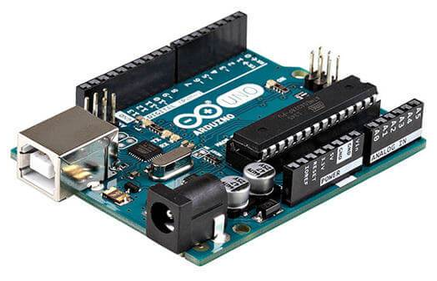
\includegraphics[width=60mm]{Chapters/images/Arduino_uno.png}}
  \subfloat[Raspberry Pi 2 Model B ]{\label{figur:2}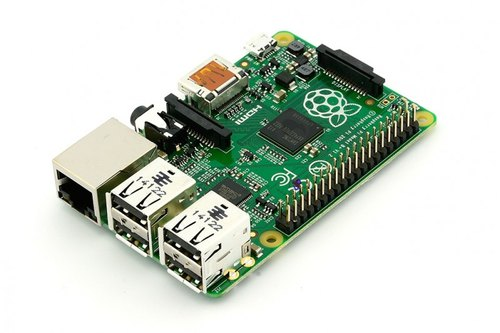
\includegraphics[width=60mm]{Chapters/images/raspeberry_modelb.jpg}}
  \setfloatalignment{b}
\end{figure}

\section{Micro-controllers and Micro-processors}
Micro-controllers and Micro-processors are common terms used in IoT and embedded systems. It is worth a while to understand the difference between them, to choose which is better to our project need.\\
Micro-controllers and micro-processors are used to execute instructions and control various units interfaced with them. However their complexity and utility can vary greatly. Micro controllers are similar to a small computer fabricated into a single Integrated Circuits (IC) . It contains a processor core, ROM, RAM, and I/O pins It does not need any external circuits to do its task. It can manage memory and other services its own. It does the job of managing units as well an performing calculations. Micro-processor, on the other hand, has only CPU inside them. It does not have RAM, ROM of its own. Processors are dedicated to perform calculations. They depend on external circuits for its peripheral like RAM, ROM to work. They are used where the task are complex and tricky. Lets summarize features.
\begin{figure}[htp]
  \centering
  \label{figure}
  \caption{Processor and Controller}
  \subfloat[Microprocessor]{\label{figur:processor}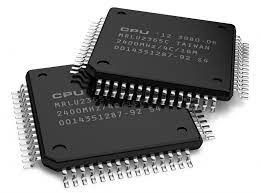
\includegraphics[width=60mm]{Chapters/images/processor.jpeg}}
  \subfloat[Microcontroller]{\label{figur:controller}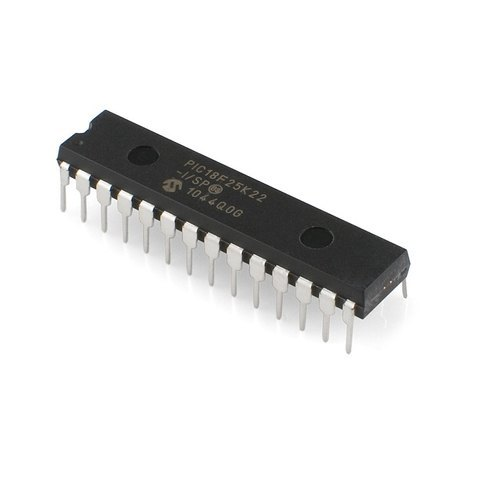
\includegraphics[width=60mm]{Chapters/images/microcontroller.jpg}}
  \setfloatalignment{b}
\end{figure}
\begin{figure}
    \centering
    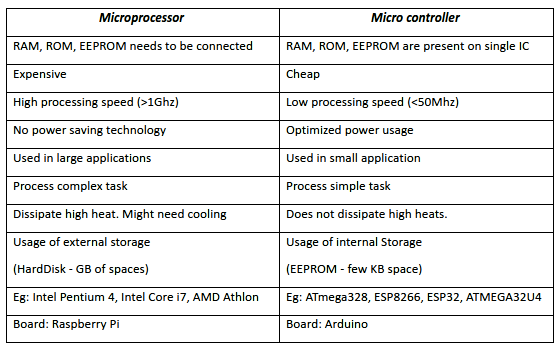
\includegraphics[width=4in]{Chapters/images/ardtab2.png}
    \caption{Comparison of Microprocessors and Microcontrollers}
    \label{fig:my_label}
     \setfloatalignment{b}
\end{figure}

\section{Arduino Boards}
Arduino is a large community that develops various micro-controller boards. Depending on the project application and usage various customized official boards are available.
\begin{figure}[htp]
  \centering
  \label{figure}
  \caption{Processor and Controller}
  \subfloat[Arduino Due]{\label{figur:processor}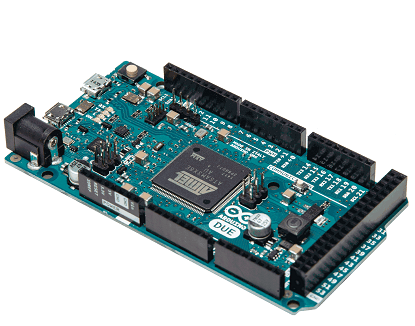
\includegraphics[width=50mm]{Chapters/images/ard1.png}}
  \subfloat[Arduino Leonardo]{\label{figur:controller}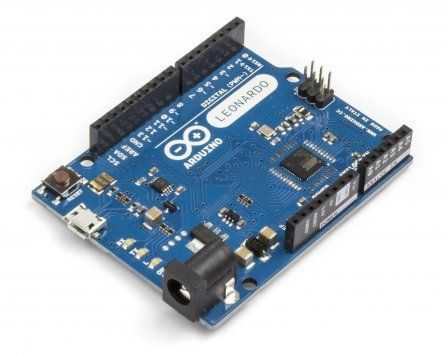
\includegraphics[width=50mm]{Chapters/images/ard2.jpg}}\\
  \subfloat[
Arduino Uno]{\label{figur:processor}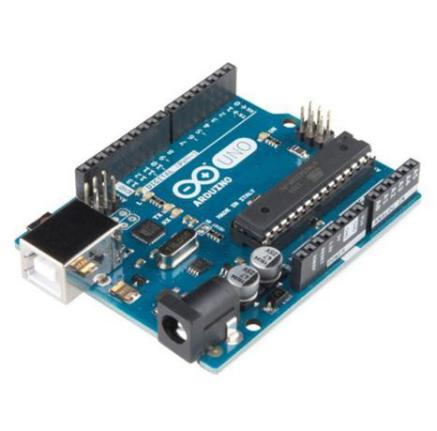
\includegraphics[width=50mm]{Chapters/images/ard3.jpg}}
  \subfloat[Arduino Mega 2560]{\label{figur:controller}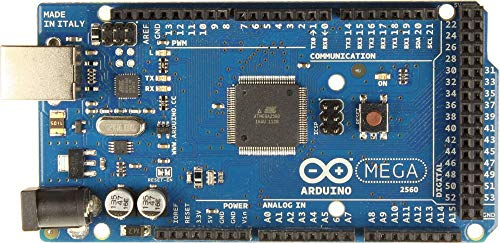
\includegraphics[width=50mm]{Chapters/images/ard4.jpg}}\\
  \subfloat[Arduino Nano]{\label{figur:processor}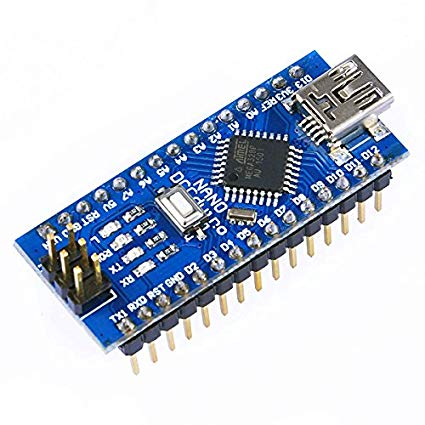
\includegraphics[width=50mm]{Chapters/images/ard5.jpg}}
  \subfloat[LillyPad Arduino]{\label{figur:controller}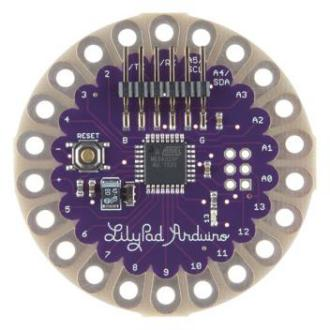
\includegraphics[width=50mm]{Chapters/images/ard6.jpg}}
  \setfloatalignment{b}
\end{figure}
\section{Arduino Uno Board}
Among various Arduino boards available, the most generally used Arduino board is the “Arduino Uno”. We would be making use of Arduino Uno to develop various projects.\\

\begin{figure}
    \centering
    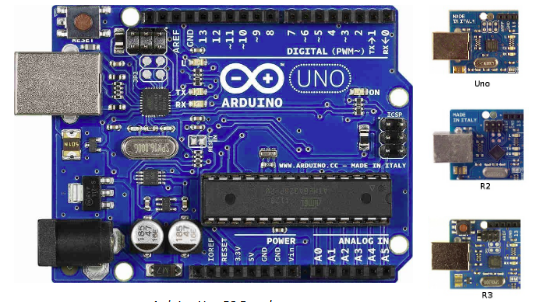
\includegraphics[width=4in]{Chapters/images/arduinor3.png}
    \caption{Arduino Uno R3 Board}
    \label{fig:my_label}
\end{figure}
\subsection{On-board units}
\begin{itemize}
    \item ATmega328 micro controller : Heart of Arduino Uno R3. This micro controller unit executes instructions. Programs are stored inside this unit.
    \item ATmega16U2 micro controller : Used to assist main micro controller. Placed near to USB port to decode USB information. Stands as a boot loader that write programs into main micro controller. The transmit LED (Tx LED) and receive (Rx LED) turns on whenever read or write operations are performed to ATmega328. 
    \item 16Mhz : Act as heart beat of Arduino board. Serves as clock for timing various units.
    \item Use type-B : Used to interface Arduino to computer. Arduino board can be programmed via USB. Serial communication with board and serial monitor can also be achieved.
    \begin{marginfigure}
     \hspace{-1in}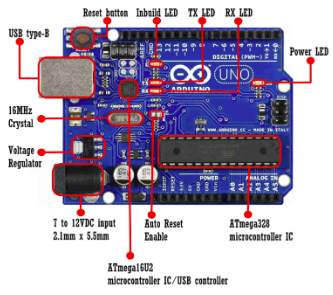
\includegraphics[width=3in]{Chapters/images/ard_boarddesp.png}
    \caption{Arduino Board Description}
    \end{marginfigure} 
    \item 12V DC input : The board can be powered via 12V DC adapter. The 12V is passed via capacitors to provide enough ampere and voltage across the board.
    \item Voltage regulator : The digital circuits usually work at 5V. The 5V voltage regulator ensures that all the units gets proper voltage levels. If the board is successfully powered, the power LED glow brightly.
    \item Reset Button : At time we might need to restart the board from the beginning. The reset button is used to reload the program from start. The reset can also be triggered inside the program.
\end{itemize}
\section{Micro controller : ATmega328}
\begin{figure}
    \centering
 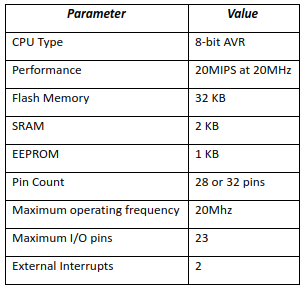
\includegraphics[width=4in]{Chapters/images/ardtab.png}
    \caption{Arduino Uno R3 Board}
    \label{fig:my_label}
\end{figure}

\section{Pin Layout : Arduino Uno}





